%!TEX root = ../main.tex
% =============================================================
%  CAPÍTULO 3 — MARCO TEÓRICO Y ESTADO DEL ARTE
%                                       (Entrega 3 · 10 % · 28/7)
% =============================================================

\chapter{Síntesis de la literatura consultada}\label{cap:marco-teorico}

\begin{guia}[Guía de la cátedra: qué se evalúa en este capítulo]
\begin{enumerate}
    \item \textbf{Estado del arte}: investigaciones nacionales,
          internacionales y productos similares, por separado. De cada
          trabajo: qué hizo y qué resultados obtuvo, con métricas.
    \item \textbf{Brechas identificadas}: qué falta en lo existente y
          justifica \emph{este} proyecto. Es lo que separa un estado del
          arte de un listado. Incluir también los resultados negativos de
          la literatura.
    \item \textbf{Bases teóricas}: desarrollan las variables del título y su
          relación. Cada concepto termina explicando cómo se usa en el
          proyecto (teoría instrumental, no de relleno). Citas canónicas
          antes que tutoriales.
    \item \textbf{Marco conceptual}: conceptos que se nombran pero no se
          desarrollan. Los términos del glosario se marcan con
          \verb|\gls{}|, por ejemplo \gls{g:mvp} y \gls{prototipo}.
    \item \textbf{Calidad bibliográfica}: papers, tesis y libros de
          editoriales serias, con datos completos. Wikipedia y blogs restan.
    \item \textbf{Entrevistas a especialistas} (si las hay): fecha, nombre,
          cargo y aporte; transcripción en el apéndice~\ref{apx:entrevista}.
\end{enumerate}
Errores que la cátedra marca: falta de coherencia interna, bibliografía
superficial, información irrelevante o redundante. Es uno de los
capítulos más extensos (orientativo: 20 a 30 páginas).
\end{guia}

\section{Estado del Arte}\label{sec:n3.1}

\subsection{Investigación Nacional}\label{sec:n3.1.1}

En el ámbito académico nacional existen antecedentes directos en análisis estático de programas y, en particular, en análisis de contaminación (taint analysis) aplicado a JavaScript. La producción más relevante proviene del Departamento de Computación de la Facultad de Ciencias Exactas y Naturales de la Universidad de Buenos Aires (FCEyN-UBA) y del Instituto de Investigación en Ciencias de la Computación (ICC, UBA-CONICET), cuyas líneas de investigación se orientan al análisis automático de programas para su comprensión, verificación y validación.

Dentro de esa línea de trabajo, \citet{balbi2023} desarrolla una investigación centrada en la inferencia automática de especificaciones de taint analysis para el lenguaje JavaScript. El trabajo parte de la premisa de que la efectividad del análisis de contaminación no depende únicamente del motor de rastreo, sino de la calidad de las especificaciones que definen qué elementos del programa constituyen puntos de entrada (sources) o de riesgo (sinks). La solución propuesta combina un método basado en aprendizaje automático con el motor de análisis estático CodeQL, empleado como infraestructura de consulta subyacente.

Esta investigación se articula con producción científica de proyección internacional. \citet{dutta2022} presentan InspectJS en el 44th International Conference on Software Engineering (ICSE-SEIP), trabajo que aborda la inferencia de especificaciones de taint para JavaScript mediante similitud de código y retroalimentación del usuario. Los autores sostienen que el mecanismo de rastreo de contaminación se implementa una única vez en el motor y luego se parametriza con distintos conjuntos de sources, sinks y sanitizers, lo que permite detectar categorías diversas de vulnerabilidades sin modificar la lógica interna del analizador. Este principio de desacoplamiento entre el motor de análisis y el catálogo de reglas constituye un fundamento directo del diseño de catálogo externo en formato JSON adoptado en el presente proyecto.

En el plano de la investigación aplicada, se registran trabajos nacionales que emplean el análisis estático como instrumento de auditoría sobre productos concretos. La Universidad Argentina de la Empresa (UADE) desarrolló una investigación orientada a evaluar las características de seguridad de videojuegos basados en NFT Gaming (2021-2022), combinando el análisis estático del código fuente en busca de vulnerabilidades con el análisis dinámico de los datos recopilados por las aplicaciones \citep{villan2022}.

Como ámbito de difusión científica, el Simposio Argentino de Ingeniería de Software (ASSE), integrado a las Jornadas Argentinas de Informática (JAIIO) organizadas por la Sociedad Argentina de Informática e Investigación Operativa (SADIO) desde 1961, constituye el foro nacional de referencia para la producción en ingeniería de software y ha sido consultado como fuente de antecedentes locales.

\subsection{Brechas Identificadas en la Investigación Nacional}\label{sec:n3.1.2}

El relevamiento de la literatura nacional permite delimitar con precisión el aporte del presente proyecto:

\paragraph{Dependencia de motores industriales preexistentes:} los antecedentes nacionales de investigación fundamental operan sobre infraestructuras de análisis ya construidas (particularmente CodeQL) y concentran su innovación en la capa de inferencia de especificaciones. La construcción propia del recorrido posterior al análisis sintáctico —la transformación del árbol en grafo de flujo de datos, su persistencia y el motor de consultas autónomo— permanece fuera del alcance de estos trabajos, que la asumen como un componente disponible.

\paragraph{Ausencia de implementaciones académicas reproducibles de extremo a extremo:} no se identifican en el ámbito nacional desarrollos académicos de código abierto que documenten e implementen de manera integral la compilación directa del código fuente a un grafo de propiedades persistido, junto con el motor de consultas de accesibilidad y un banco de pruebas reproducible por terceros.

\paragraph{Orientación aplicada desacoplada del diseño del analizador:} los trabajos de investigación aplicada locales emplean herramientas comerciales o de código abierto existentes como instrumentos de auditoría sobre software final, sin abordar el diseño algorítmico del motor de detección ni la evaluación cuantitativa de su precisión frente a enfoques alternativos.

\paragraph{Escasa exploración de la visualización topológica del riesgo:} la representación interactiva del recorrido del dato contaminado sobre la topología del programa, orientada a reducir el esfuerzo de interpretación del hallazgo por parte del equipo de desarrollo, no aparece tratada como objeto de estudio en los antecedentes nacionales relevados.

\subsection{Investigaciones Internacionales}\label{sec:n3.1.3}

A nivel internacional, la representación del código mediante grafos y el análisis de flujo de datos cuentan con antecedentes teóricos y empíricos fundamentales:

\paragraph{Code Property Graphs (CPG):} \citet{yamaguchi2014} formalizaron la representación unificada del código fuente combinando en una misma estructura de grafo el Árbol de Sintaxis Abstracta (AST), el Grafo de Flujo de Control (CFG) y el Grafo de Dependencia de Datos (DDG). Este trabajo mostró que la detección de vulnerabilidades puede expresarse como un problema de consulta de accesibilidad sobre grafos.

\paragraph{Object Dependence Graphs (ODG):} \citet{li2022} desarrollaron un modelo basado en grafos de dependencia de objetos para detectar vulnerabilidades en el ecosistema Node.js / JavaScript, demostrando que el rastreo de objetos en lenguajes dinámicos permite abordar patrones de riesgo no detectados por el análisis estático convencional.

\paragraph{Estudios comparativos de herramientas SAST en Node.js:} \citet{brito2023} evaluaron empíricamente la efectividad de herramientas de análisis estático sobre paquetes reales del ecosistema Node.js, caracterizando sus limitaciones de cobertura y precisión.

\subsection{Productos Similares}\label{sec:n3.1.4}

En la industria del software existen herramientas consolidadas que aplican principios de análisis de flujo de datos e inspección de código:

\begin{table}[H]
    \centering
    \caption{Comparación de herramientas SAST similares}
    \label{tab:comparativa}
    \small
    \begin{tabularx}{\textwidth}{l L L L}
        \toprule
        \tb{Herramienta} & \tb{Motor de Análisis} & \tb{Alcance y Enfoque} & \tb{Diferenciación con GraphSAST} \\
        \midrule
        CodeQL (GitHub / Semmle) & Motor relacional basado en grafos interpretados con lenguaje declarativo QL. & Plataforma profesional multilenguaje de alcance industrial. & Requiere infraestructura y compilación pesada; GraphSAST implementa un motor liviano enfocado en TypeScript/JavaScript con persistencia nativa en base de datos de grafos y visualización web interactiva. \\
        Semgrep & Motor de coincidencia de patrones sintácticos abstractos con soporte de taint mode. & Análisis rápido en pipelines de CI/CD basado en reglas declarativas en YAML. & Su enfoque principal es la ejecución de reglas en línea de comandos; no persiste la topología completa del programa en una base de datos de grafos para consultas de arquitectura. \\
        Joern & Plataforma de código abierto basada en Code Property Graphs (CPG). & Análisis estático avanzado enfocado en C/C++ y Java utilizando la base OverflowDB. & Orientado a análisis por consola mediante entorno REPL (Scala); GraphSAST simplifica la inspección mediante un panel web con renderizado dinámico de nodos. \\
        \bottomrule
    \end{tabularx}
\end{table}

\section{Marco Teórico}\label{sec:n3.2}

En consonancia con la metodología académica establecida, se definen en primer lugar las variables de investigación y su relación teórica:

\paragraph{Variable independiente ($V_1$).} representación del código fuente mediante grafos de flujo de datos (Data Flow Graphs).

\paragraph{Variable dependiente ($V_2$).} detección estática de vulnerabilidades de arquitectura de software y precisión en el análisis de contaminación (Taint Analysis).

\paragraph{Relación entre las Variables:} la hipótesis central de este trabajo sostiene que transformar la estructura sintáctica del código fuente en una representación matemática en forma de grafo dirigido permite formular la detección de vulnerabilidades como un problema formal de accesibilidad (reachability), mejorando la precisión y reduciendo la tasa de falsos positivos en comparación con los analizadores estáticos basados en coincidencia de patrones de texto.

\subsection{Análisis Estático de Código Fuente (SAST) y \enquote{Building Security In}}\label{sec:n3.2.1}

El análisis estático de código fuente consiste en la evaluación del código de una aplicación sin requerir su ejecución dinámica \citep{nielson1999}. En la ingeniería de software, \citet{mcgraw2006} formalizó el principio de incorporar prácticas de seguridad de manera intrínseca desde las fases iniciales del ciclo de vida del desarrollo de software (SDLC), enfoque que la industria denominaría posteriormente bajo el término Shift-Left Security. Detectar y corregir defectos de diseño y vulnerabilidades durante la fase de codificación evita que la deuda técnica de seguridad se propague hacia los entornos de prueba o producción, reduciendo los costos de remediación.

\subsection{Compiladores, Análisis Léxico, Parsing y Árboles de Sintaxis Abstracta (AST)}\label{sec:n3.2.2}

La teoría clásica de compiladores establece que el procesamiento del código fuente comienza con la fase de análisis léxico (scanning), donde la secuencia lineal de caracteres se convierte en una serie de tokens, seguida por el análisis sintáctico (parsing), que construye una representación jerárquica denominada Árbol de Sintaxis Abstracta (Abstract Syntax Tree - AST) \citep{aho2006}. El AST representa la estructura gramatical del programa en forma de árbol.

En el marco de este proyecto, el proceso de parsing se fundamenta en la API del compilador oficial de TypeScript a través de la biblioteca ts-morph. Esta herramienta permite consumir código fuente escrito en JavaScript/TypeScript y extraer una representación estructurada compuesta por nodos sintácticos (tales como declaraciones de funciones, asignaciones de variables, llamadas a métodos e identificadores).

\subsection{Representación del Código mediante Grafos: Call Graph y Data Flow Graph (DFG)}\label{sec:n3.2.3}

Aunque el AST proporciona la estructura sintáctica del programa, no modela de forma explícita las relaciones de dependencia ni el recorrido de los datos a través de las diferentes funciones y módulos \citep{yamaguchi2014}. Para superar esta limitación, la literatura propone construir dos representaciones sobre el AST:

\paragraph{Call Graph (Grafo de Invocaciones):} grafo dirigido donde los nodos corresponden a funciones o métodos y las aristas dirigidas representan llamadas efectivas entre ellos, permitiendo realizar un análisis tanto intraprocedural (dentro de una misma función) como interprocedural (entre distintos archivos y módulos).

\paragraph{Data Flow Graph - DFG (Grafo de Flujo de Datos):} grafo dirigido $G = (V, E)$ donde el conjunto de vértices $V$ representa variables, operaciones e identificadores, y el conjunto de aristas dirigidas $E$ modela la propagación y mutación de los valores.

En la fundamentación de este trabajo, el Grafo de Flujo de Datos formaliza las relaciones entre nodos mediante los siguientes tipos de aristas dirigidas:

\begin{itemize}
    \item \textbf{FLOWS\_TO:} indica la transferencia o asignación directa del valor de una variable a otra.
    \item \textbf{CALLS:} representa la invocación de una función o método con paso de parámetros.
    \item \textbf{BINDS\_TO:} modela la vinculación semántica entre parámetros formales y argumentos reales.
    \item \textbf{RETURNS:} representa el retorno de un valor desde el ámbito de una función hacia el contexto invocador.
    \item \textbf{SANITIZED\_BY:} modela la intercepción y neutralización del dato por parte de una función de validación o limpieza.
\end{itemize}

\begin{figure}[H]
    \centering
    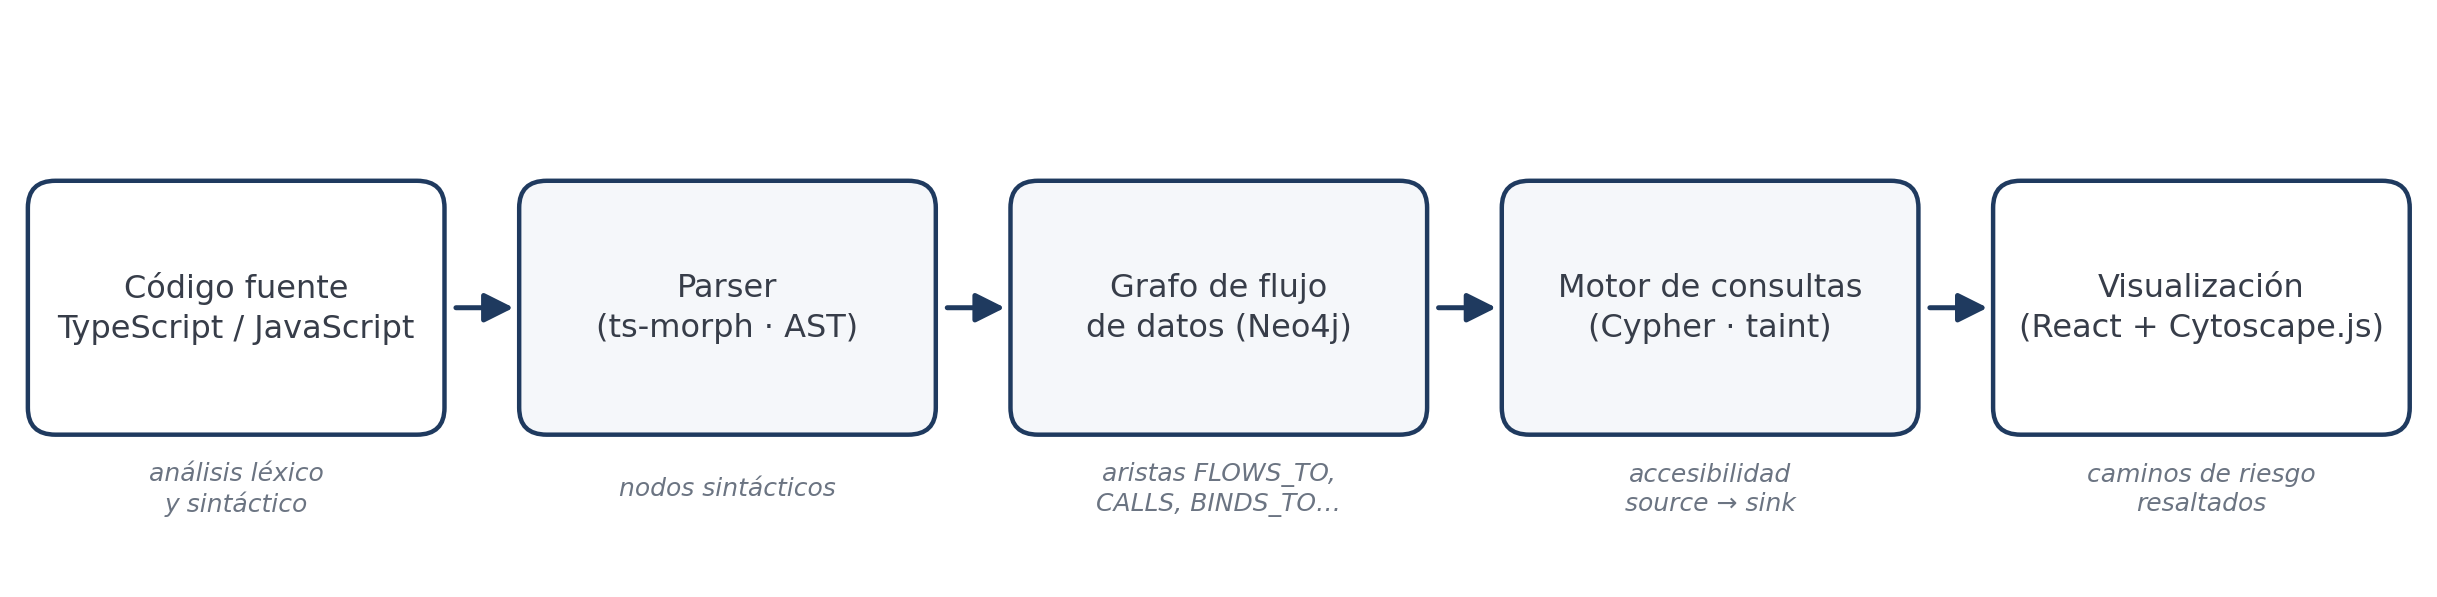
\includegraphics[width=\textwidth]{figuras/flujo-general.png}
    \caption{Flujo general de procesamiento de GraphSAST: código fuente, parser, grafo de flujo de datos, consultas y visualización}
    \label{fig:flujo-general}
\end{figure}

\subsection{Análisis de Contaminación (Taint Analysis)}\label{sec:n3.2.4}

El análisis de contaminación (taint analysis) es un método formal fundamentado en la teoría del flujo de información \citep{denning1976,sabelfeld2003,nielson1999} para verificar si datos provenientes de fuentes no confiables pueden alcanzar operaciones sensibles sin una sanitización intermedia adecuada. El modelo teórico se define mediante la tupla $(S, K, F)$:

\paragraph{Source ($S$, origen).} conjunto de nodos que representan puntos de entrada de información externa al programa no controlada por el sistema (por ejemplo, parámetros HTTP req.body, req.query, o entradas de usuario).

\paragraph{Sink ($K$, destino).} conjunto de nodos que representan operaciones o funciones críticas donde la utilización de un dato no seguro genera una vulnerabilidad (por ejemplo, consultas SQL db.query(), ejecución de comandos child\_process.exec(), o renderizado en interfaz).

\paragraph{Sanitizer ($F$, sanitizador).} conjunto de nodos u operaciones que aplican filtros, codificaciones o validaciones que remueven la condición de contaminación del dato.

Desde la perspectiva de la teoría de grafos, una vulnerabilidad de seguridad se define formalmente como un problema de accesibilidad (reachability): existe una vulnerabilidad si y solo si en el grafo $G$ existe un camino dirigido $p = (v_1, v_2, \ldots, v_n)$ tal que $v_1 \in S$, $v_n \in K$ y $\forall v_i \in p,\ v_i \notin F$.

\begin{figure}[H]
    \centering
    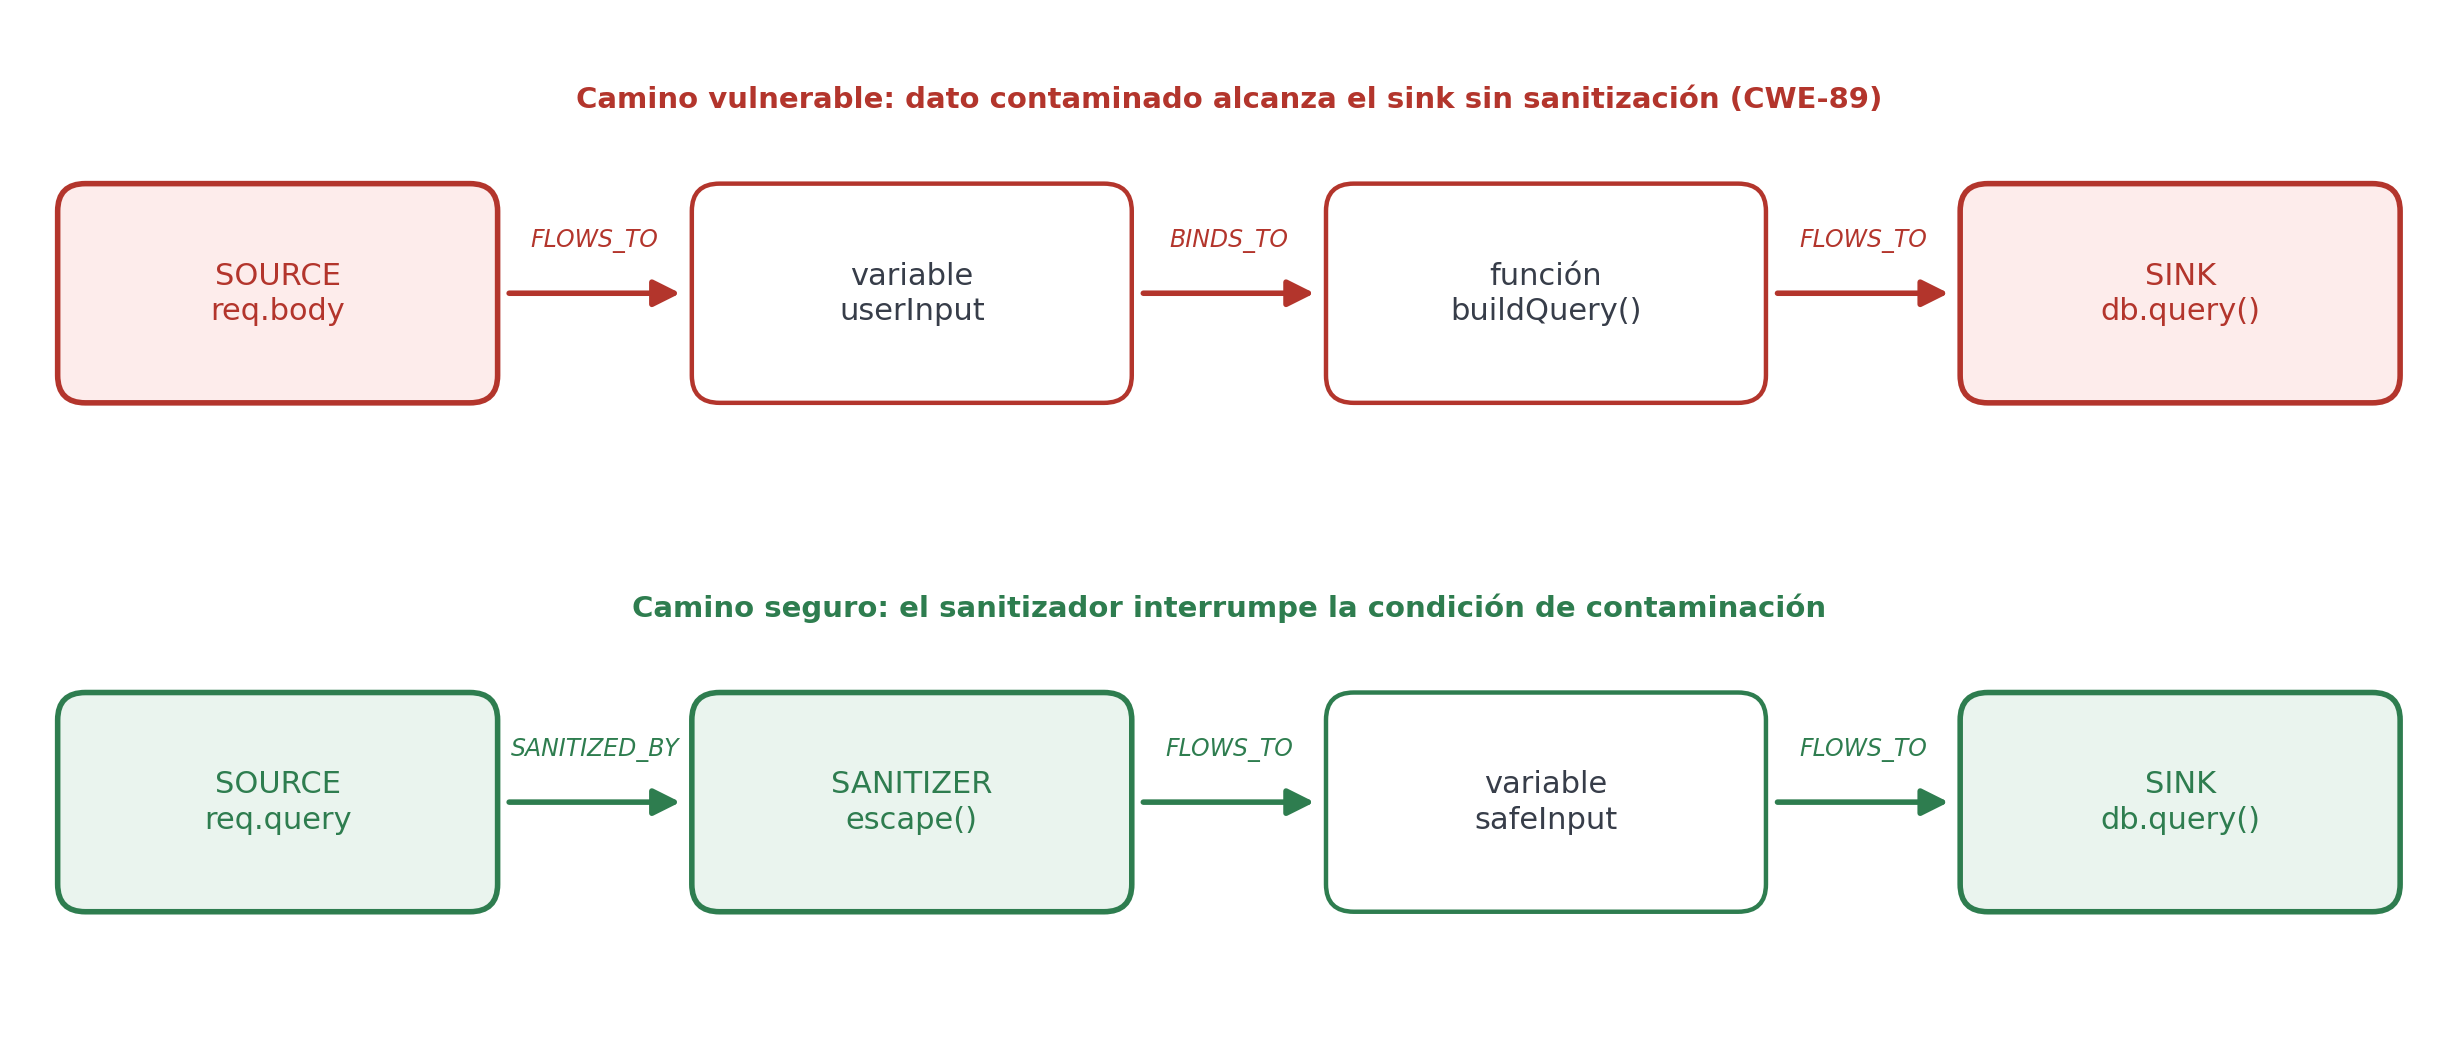
\includegraphics[width=0.9\textwidth]{figuras/source-sink.png}
    \caption{Recorrido source-sink utilizado en el análisis de taint}
    \label{fig:source-sink}
\end{figure}

\subsection{Bases de Datos Orientadas a Grafos y Motor de Consultas (Neo4j y Cypher)}\label{sec:n3.2.5}

Una base de datos orientada a grafos es un sistema de gestión de bases de datos diseñado para almacenar y consultar estructuras de red compuestas por nodos, aristas y propiedades \citep{robinson2013}. Su ventaja técnica fundamental frente a las bases de datos relacionales en la ejecución de recorridos locales reside en la propiedad de adyacencia sin índices (index-free adjacency), donde cada nodo mantiene referencias directas hacia sus nodos vecinos, permitiendo explorar caminos sin realizar operaciones costosas de cruce (joins).

Para la aplicación en este proyecto, se adopta Neo4j como motor de persistencia del grafo compilado y el lenguaje Cypher como motor de consultas declarativo. Cypher permite expresar patrones de accesibilidad de longitud variable entre nodos de tipo Source y Sink, recorriendo de forma combinada las relaciones de flujo de datos, invocación, vinculación de parámetros y retorno, y descartando aquellos caminos en los que interviene una operación de sanitización.

\subsection{Catálogo de Vulnerabilidades de Arquitectura (CWE)}\label{sec:n3.2.6}

La clasificación de vulnerabilidades se fundamenta en el estándar internacional Common Weakness Enumeration (CWE) de la organización MITRE \citep{mitrecwe}. En este trabajo, el motor de detección se enfoca en tres patrones de riesgo arquitectónico:

\paragraph{CWE-89 (SQL Injection):} ocurre cuando datos no sanitizados de una source fluyen hacia la construcción de consultas SQL dinámicas en un sink de base de datos.

\paragraph{CWE-79 (Cross-Site Scripting - XSS):} ocurre cuando datos no confiables alcanzan salidas del navegador o respuestas HTTP sin la debida codificación.

\paragraph{CWE-78 (Command Injection):} ocurre cuando entradas externas fluyen hacia funciones de ejecución de comandos del sistema operativo (exec, spawn).

\subsection{Visualización de Software e Interfaz Interactiva de Grafos}\label{sec:n3.2.7}

La disciplina de visualización de software (Software Visualization) sostiene que la representación gráfica interactiva de las estructuras y flujos internos del programa reduce la carga cognitiva en la comprensión de la arquitectura y la identificación de fallas \citep{diehl2007}. La integración de herramientas de renderizado de grafos como Cytoscape.js en entornos web modernos permite transformar los hallazgos de seguridad en diagramas interactivos donde los caminos críticos Source $\rightarrow$ Sink se resaltan sobre la topología del código, facilitando el diagnóstico por parte del desarrollador.

\section{Marco Conceptual}\label{sec:n3.3}

\subsection{Vulnerabilidad de Arquitectura}\label{sec:n3.3.1}

Defecto de seguridad cuya existencia no se manifiesta en una sentencia aislada del código, sino en la forma en que los componentes del sistema se vinculan entre sí y en el recorrido que la información describe a través de ellos. A diferencia de las vulnerabilidades localizadas —identificables mediante la inspección de una única línea o expresión—, una vulnerabilidad de arquitectura requiere reconstruir la propagación del dato a través de múltiples funciones, módulos o capas de abstracción para poder ser detectada. Su identificación exige, en consecuencia, una representación del programa que exceda el ámbito de la sentencia individual.

\subsection{Deuda Técnica de Seguridad}\label{sec:n3.3.2}

Especialización del concepto de deuda técnica que cuantifica el costo diferido y el riesgo acumulado en un sistema de software debido a decisiones de diseño o deficiencias de seguridad no resueltas en el código fuente. Una alta deuda técnica de seguridad incrementa la superficie de ataque del sistema.

\subsection{Indicadores de Calidad del Analizador: Precisión, Exhaustividad, Falsos Positivos y Negativos}\label{sec:n3.3.3}

Conjunto de métricas estadísticas utilizadas para medir el desempeño de un sistema SAST:

\paragraph{Falso positivo (FP).} alerta reportada por el analizador sobre un fragmento de código que en realidad es seguro o está correctamente sanitizado.

\paragraph{Falso negativo (FN).} vulnerabilidad real presente en el código fuente que el analizador omite detectar.

\paragraph{Precisión (Precision):} proporción de vulnerabilidades reales detectadas sobre el total de alertas emitidas por la herramienta:

\[ \mathit{Precision} = \frac{TP}{TP + FP} \]

\paragraph{Exhaustividad (Recall):} proporción de vulnerabilidades reales detectadas sobre el total de vulnerabilidades existentes en el programa:

\[ \mathit{Recall} = \frac{TP}{TP + FN} \]

\subsection{Accesibilidad (Reachability) en Grafos Dirigidos}\label{sec:n3.3.4}

Propiedad matemática de la teoría de grafos que determina si existe una secuencia de aristas dirigidas que conecte un nodo de origen $u$ con un nodo de destino $v$. En el contexto del análisis estático, se utiliza para verificar formalmente si existe flujo de información entre dos puntos del programa.

\subsection[Sensibilidad en el Análisis de Programas]{Sensibilidad en el Análisis de Programas\newline (Flow-, Context- y Path-Sensitivity)}\label{sec:n3.3.5}

Clasificación teórica que define el grado de precisión y el nivel de abstracción adoptado por un algoritmo de análisis estático \citep{nielson1999}:

\paragraph{Sensibilidad al Flujo (Flow-sensitivity):} un análisis es sensible al flujo si tiene en cuenta el orden de ejecución de las sentencias del programa. Un análisis insensible al flujo considera las sentencias como un conjunto no ordenado.

\paragraph{Sensibilidad al Contexto (Context-sensitivity):} un análisis es sensible al contexto si distingue entre las diferentes invocaciones de una misma función según la pila de llamadas (call stack) desde donde fue emitida, evitando mezclar los flujos de datos de distintas llamadas.

\paragraph{Sensibilidad al Camino (Path-sensitivity):} un análisis es sensible al camino si evalúa la validez de los predicados o condiciones lógicas de las ramificaciones (if, switch), diferenciando rutas de ejecución factibles de aquellas que son inalcanzables.
